\documentclass[review]{elsarticle}

\usepackage{amsmath,amssymb}
\usepackage{mathtools}
\usepackage{tensor}
\usepackage{adjustbox}
\usepackage{multirow}
\usepackage{threeparttable}
\usepackage[utf8]{inputenc}
\usepackage{booktabs, caption, makecell}
\usepackage{tikz}
\usetikzlibrary{arrows.meta,positioning}
\usepackage[labelfont=bf]{caption} % Package to create caption to the figures


\usepackage{lineno,hyperref}
\modulolinenumbers[5]
\allowdisplaybreaks


% This avoid a foot note about to which paper the article was submited
\makeatletter
\def\ps@pprintTitle{%
 \let\@oddhead\@empty
 \let\@evenhead\@empty
 \def\@oddfoot{}%
 \let\@evenfoot\@oddfoot}
\makeatother

%%%%%%%%%%%%%%%%%%%%%%%
%% `Elsevier LaTeX' style
\bibliographystyle{elsarticle-num}
%%%%%%%%%%%%%%%%%%%%%%%

\begin{document}

\begin{frontmatter}

\title{Intertemporal logistics collaboration \\[5pt]
                \normalsize{Msc Thesis}}

%% Group authors per affiliation:
\author{Antón de la Fuente suárez-Pumariega}
\address{a.delafuentesuarez-pumariega@student.maastrichtuniverisry.nl }

%% or include affiliations in footnotes:
\author{Maastricht Univeristy}



\begin{abstract}
Here goes the abstract
\end{abstract}

\begin{keyword}
Here\sep go \sep KEY \sep words
\end{keyword}

\end{frontmatter}

% Desactivation of numbering every 15 LINES
%\linenumbers

\section{Introduction}

During the last decades, logistics collaboration, and specially \emph{horizontal
logistics collaboration}, has gained the attention of many researchers, as it
has been proofed to be an effective strategy to improve the logistics chain, for
example, reducing both ecological and economical 
costs \cite{BALLOT2010} \cite{SOYSAL2018168}. By horizontal logistics collaboration we refer to the
cooperation between several companies or agents, who playing the same role in
the logistics chain, form coalitions or alliances to increase the efficiency of
their logistics operations. For example, in the case of the liner hipping
industry, by allowing other companies to use part of the capacity of the own
ships, increasing the asset utilization ratio \cite{AGARWAL2008175}.

The literature studying the horizontal logistics collaboration between agents
can be divided in two main streams depending on whether the collaboration it is
centralized or decentralized. In this first case, the common approach is to give all the power to a central planner, who manages all the assets and demands of a coalition of agents and then some allocation rule is used to allocate the benefit generated. In the second one, auctions were agents can exchange demands are frequentlly used. One important difference among this two approaches is that in the decentralized one, agents remain independent decision makers.

In this paper we explore different cooperation mechanisms in the context of the horizontal logistics collaboration between courier companies, modelling the optimization problem they have to solve as a network-design multicommodity flow problem. In section \ref{seq:litreview} we develop a review on the literature we studied during the development of this work. In section \ref{seq:probdefinition} we define the problem and present the model for a single agent. Section \ref{seq:centrmodels} contains three different centralized cooperation mechanism. In section \ref{seq:itermodel} we introduce a, to best of our knowledge, novel approach to model a decentralized cooperative mechanism. Section \ref{seq:results} contains the results of the simulations we have done with the models presented in the two previous section. Section \ref{seq:discussion} is a discussion about the limitations and possible extensions of the models proposed in this paper. We finish with a conclusion in section \ref{seq:conclusion}.



\section{Literature review}\label{seq:litreview}

The literature studying the horizontal logistics collaboration between agents
can be divided in two main streams depending on whether the collaboration it is
centralized or not.

\subsection{Centralized cooperation}

In the case of centralized systems, agents usually share in a pool all or
part of the demands that they have to serve as well as the assets they have
available. These assets can be vehicles in the case of transportation carriers,
but also inventory levels, employees, etc. Then a central planner, taking into
account all the demands and sources shared in the pool by the agents, solves the
problem maximizing the total payoff of the coalition. Finally, the benefits of
the cooperation are shared among the members of the coalition, usually using
some allocation rule which ideally satisfies some desirable conditions in
terms of ``fairness'', as that the resulting allocation is in the \emph{core},
i.e., any subcoalition of the former one could obtain a higher payoff working
independently \cite{GONZALEZ2010}. A well known example of an allocation rule
fulfilling this conditions is the \emph{Shapley value} \cite{SHAPLEY1952}.

Some authors have pointed that in the centralized systems, the individual objectives
of the agents are often not considered in favour of the coalition objective, what neglects the fact that the agents actually remain independent entities \cite{DEFRYN2018891}. Therefore,
these authors propose different mechanisms where both levels of objectives are
considered \cite{DEFRYN20191} \cite{VANOVERMEIRE2014125}. Furthermore, it is assumed
in the literature studying these type of systems that agents share all their private information
with the central planner, what might be unrealistic or problematic in real world cases \cite{SERRANO2017} \cite{ZENG2015}.


\subsection{Decentralized cooperation}

Some decentralized cooperative mechanism operate based on auctions systems. In that systmem, agents share
the part of their demands, an the other members of the coalition bid to be the
ones serving that demand, for what the obtain some benefit \cite{LEDYARD2002} \cite{MAHR201099}. Non-auction based decentralized systems have also been stuy \cite{HERNANDEZ2014} \cite{WANG2014} . Nevertheless, in this works there is still a central authority which has to make some decisions. We refer the reader to \cite{GANTERER2017} for a survey covering decentralized mechanism based and not based in auctions.

A collaborative system based in a
inverse-optimization mechanism is the proposed in \cite{AGARWAL2008520}. On it,
the authors model a multicommodity flow problem, where agents own certain
fraction of the capacity of the edges of a network. Thus, the agents can
collaborate sharing the capacity of the edges with the members of the coalition,
who have to pay some price for using that edges. How much capacity the agents
own on each edge of the and which are their demand is assumed to be public
information. Using inverse optimization, capacity exchange prices are
found, in such a way that if the agents adopt that prices policy, when each
agent selfishly optimizes his demands through the shared network, the resulting
flow will be the same that if a centralized approach was used. However, we argue that might be difficult or even unrealistic to implement in the real work a cooperation mechanism were a central authority with full information impose the prices at which the agents can exchange assets.

In \cite{ANUPINDI2001} a novel framework to model decentralized systems is proposed. Based in the concept of \emph{coopetition} \cite{BRANDENBURGER1996},
the authors proposed a 2-stage mechanism to model the collaboration of agents in
decentralized distribution systems. In the first stage, agents individually
take strategic decisions, in their case, fixing their inventory levels. In the
seconds stage and after all the agents have served their demands in the best way they individually can, they cooperate sharing their residual demands and inventory with the others, obtaining
extra profits. They propose sufficient conditions under which a Nash equilibrium
in pure strategies exist for the first stage, and for which an allocation rule in
the \emph{core} exists for the second stage.




In this work we analyse and compare several centralized systems,
giving to central planner different degrees of decision power, and a non-auction-based decentralized system, where we substitute the central planner by a platform where agents can share information, and through an iterative process of optimization
and information sharing, similar to what is done in \cite{WANG2014} but without leaving any decision power to the platform, agents can achieve an equilibrium point from which no agent would be interested to unilaterally deviate from. The problem we
will use as example to implement this models is a multicommodity flow problem,
where each agent have to decide which edges to active on the network at certain
price, to then find an efficient flow through them which maximizes their
payoff.

\section{Problem statement: A network design - muldicommodity flow problem}\label{seq:probdefinition} 

As stated in the previous section, we will use a multicommodity flow problem
with a network design stage to illustrate the different cooperation
mechanisms we study in this paper. In the problem we propose, a simplified version of the one studied in \citep{AGARWAL2008175}, a set of agents have
to first decide which edges they want to activate in a network, with certain
costs associated. Then, each have to route their commodities through the edges
he has activate. The objective of the agents is to maximize the revenues generated by the served commodities and minimize the costs associated with the activation of the edges. This two subproblems are intrinsically linked: the most efficient flow an agent can find for his commodities depends on which edges he has access too, and to know which edges to activate, the agent need to know how he will route his commodities through that edges. 

The agents can collaborate among them sharing the capacity they do not use in their active edges, allowing others to route their commodities through them at some price. 

% On the rest of this section we will introduce the specific characteristics of these problem as well as the notation we will use. We will finish the section modelling the problem that each agent would face in case he does not take part of the collaboration.

Let $N=\{1,...,n\}$ be a set of agents. Let $G=(V,E)$ be a directed graph with
$V$ and $E$ the sets of nodes and edges respectively. 
Let $\Theta$ be the set of commodities. Each commodity is noted by a tuple,
$(o,t,i)$, where $o\in V$ is its origin node, $t\in V$ its destiny node and $i$
is the agent who owns it. A commodity $(o,t,i)$ has a size of $d_{(o,t,i)}$ units and has an associated revenue $r_{(o,t,i)}$. The owner of the commodity $(o,t,i)$ earns $d_(o,t,i)\cdot r_(o,t,i)$ if the commodity is successfully delivered from its origin to its terminal node. The commodities are unsplitable, i.e., can not be divided between different edges. Each edge $e \in E$ will be noted by a tuple, $e=(v,w,i)$, indicating that it connects the node $v\in V$
with the node $w \in V$ and that his owner is the agent $i\in N$. Note that
could exist as many edges between a pair of nodes as agents exists. Each edge $e
\in E$ has certain units of capacity associated $q_e$, and a a fixed activation
cost $c_e$, that the owner of the edge have to pay if he wants to use the edge to route any commodity. We will note by $OE(v)\subset E$ the subset of edges whose origin is the node $v\in V$. Similarly, $IE(v)\subset E$ is the subset of edges whose terminal node is $v\in V$.

We will note by $E^i \subset E$ and $\Theta^i\subset \Theta$ the subsets of
edges and commodities owned by agent $i$.

\begin{table}[ht!]
	\caption{Summary of notation \label{tb:notation}}
	\begin{tabular}{|l|l|}
	\hline
	Symbol & Meaning	 \\ \hline
	$N$ & Set of agents. \\
	$G$ & Network. \\
	$V$ & Set of nodes in $G$. \\
	$E$ & Set of edges in $G$. \\
	$\Theta$ & Sets of commodities. \\
	$\delta^+(v)$ & Subset of edges in $E$ which depart from node $v$.\\
	$\delta^-(v)$ & Subset of edges in $E$ which arrive to node $v$.\\	
	$\Theta^i$ & Set of commodities owned by agent $i$. \\	
	$E^i$ & Set of edges owned by agent $i$.\\
	$E_A$ & Subset of edges in $E$ that are active \\
	$E_R$ & Subset of edges in $E_A$ that have residual capacity.\\
	\multirow{2}{*}{$(o,t,i)\in \Theta$} & Commodity with origin node $o$ and terminal node $t$\\[-3pt]
	& owned by agent $i$. \\
	$d_{(o,t,i)}$ & Size, on units, of commodity $(o,t,i)$.\\
	$r_{(o,t,i)}$ & Revenue associated with serving commodity $(o,t,i)$.\\
	$e=(v,w,i)\in E$ & Edge connecting node $v$ with node $w$, owned by agent $i$.\\
	$c_e$ & Cost of activate edge $e$. \\
	$q_e$ & Units of capacity of edge $e$. \\
	$q_e^R$ & Units of residual capacity of edge $e$.\\
	\hline
	\end{tabular}
\end{table}

\subsection{Single agent model}

The objective of an agent $i \in N$ is to maximize his payoff, by routing his
commodities, $\Theta^i$, from their origin nodes to their terminal nodes through the edges $E^i$, he has activated. If the agent does not take part of the collaboration, she will not have any access to other agents edges, neither the other agents can route their commodities through his edges. Thus, the problem which agent $i\in N$ has to solve can be modelled as the following ILP, that we call $P_i$,

    \begin{align}
        &  P_i: \quad \max  &  \sum_{(o,t,i)\in \Theta^i} \sum_{e \in \delta^+(t)\cap E^i} f_e^{(o,t,i)} \cdot d_{(o,t,i)} \cdot r_{(o,t,i)} - \sum_{e\in E^i} u_{e'}\cdot c_{e} \hspace{20pt} &&   \label{eq:SingleAgentA}
    \end{align}
    \begin{align}
        & \text{subject to:}       &  \nonumber\\
       & \sum_{e \in \delta^-(t)\cap E^i} f_e^{(o,t,i)}-\sum_{e \in \delta^+(t)\cap E^i} f_{e}^{(o,t,i)} = 0,\quad && \forall\ z\in V\setminus\{o,t\},\ \forall\ (o,t,i)\in\Theta^i,  \label{eq:SingleAgentB}\\
        &    \sum_{e \in \delta^+(t)\cap E^i} f_e^{(o,t,i)} \leq 1,  && \forall\ (o,t,i)\in \Theta^i, \label{eq:SingleAgentC} \\
		& \sum_{e \in \delta^+(t)\cap E^i} f_e^{(o,t,i)}= 0,  && \forall\ (o,t,i)\in \Theta^i, \label{eq:SingleAgentD} \\
		& \sum_{(o,t,i) \in \Theta^i} f_e^{(o,t,i)}\cdot d_{(o,t,i)} \leq u_e\cdot q_e, && \forall\ e \in E^i,\label{eq:SingleAgentE}  \\
		& \sum_{\substack{(v,w,k) \in E^i\colon \\ v,w \in S}} f_{(v,w,i)}^{(o,t,i)} \leq |S| -1,   && \forall\ S \subset V,\ \forall\ (o,t,i) \in \Theta^i, \label{eq:SingleAgentF}\\[1em]
		& f_e^{(o,t,i)} \in \{0,1\},    && \forall\ e \in E^i,\ \forall\ (o,t,i) \in \Theta^i, \label{eq:SingleAgentG} \\ 
		&  u_e   \in \{0,1\},           && \forall\ e \in E^i 
    \end{align}

where, $\forall\ (o,t,i)\in \Theta^i$ and  $\forall\ e \in E$,
\[
\begin{array}{rl}
f_e^{(o,t,i)} = & \begin{cases}
    1 & \text{if } (o,t,i) \text{ is routed through } e,\\
    0 & \text{otherwise}
\end{cases}  \\[20pt]
u_e = &\begin{cases}
    1 & \text{if } e \text{ is activated},\\
    0 & \text{otherwise}    
\end{cases}
\end{array}
\]

The objective of agent $i$, equation (\ref{eq:SingleAgentA}), is to maximize the
profit generated by the commodities which arrive to their destination nodes
while minimizing the cost associated to the activation of the edges. Constraint
(\ref{eq:SingleAgentB}) ensure that, for any commodity, the flow that enters
and leaves every transit nodes (neither the origin, neither the terminal node of
that commodity) is equal. Constraint (\ref{eq:SingleAgentC}), together with
(\ref{eq:SingleAgentG}), guarantee that each commodity is send at most only once
from its origin node. Constraint (\ref{eq:SingleAgentD}) ensure that no
commodity is send from its terminal node to any other node. Constraint (\ref{eq:SingleAgentE})
ensures that the capacity of edges is not exceed. Finally, constraint
(\ref{eq:SingleAgentF}) is a subtour elimination constraint \cite{AHUJA1993}. We have included it in our model because, first of all, it makes sense to assume that an agent would not want to create subtours when routing his commodities. Note that subtours could be possible without this constraint because once an edge is activated, there is no extra costs for routing more commodities through it. Furthermore, without the subtour elimination constraints, the other constraints are not sufficient to ensure that all the feasible solution of the ILP are admissible, since the flow of a commodity could contain a subtour disconneted from the origin and terminal nodes of that commodity, without impacting the objective but making the solution not valid for the problem we are modelling.

We will note by $P_i^*$ the optimal solution of $P_i$ which is the maximal
payoff agent $i$ can obtain by his own without cooperating with the other agents.

\section{The centralized cooperation models} \label{seq:centrmodels}

In the previous subsection, we have presented an ILP that models the network design - multicommodity flow problem of an agent $i\in N$ who works alone. In this section, we present different centralized cooperative scenarios, where the agents in $N$ collaborative in different ways in order to find synergies among them and increase their payoffs.

In all the three different scenarios we propose, the way in which agents is sharing the capacity of the edges they have activate with other agents, what could allow to some agents to serve commodities in a cheaper way to some agents, and to compensate the cost of the activation of some edges to others. The three scenarios also have in common the way in which the agents share the benefits generated by the collaboration, what is done as follows
\begin{enumerate}
    \item The revenues generated by any served commodity are
    allocated to its owner.
    \item The activation cost of any active edge is paid by its owner.
    \item If a commodity $(o,t,i)\in \Theta$ is routed through an edge $e=(v,w,j)		\in E$ and $j\not = i$, agent $i$ makes a side payment equal to $d_{(o,t,i)})		\cdot\frac{c_e}{q_e}$ to the agent $j$. In words, for each commodity sent 		through an edge owned by other agent, the owner of the commodity will pay to 		the owner of the edge the fraction of the activation cost of that edge 			equivalent 	to the fraction of the total capacity of the edge that his 			commodity occupies.
\end{enumerate}

In the rest of the section we introduce the three different centralized
cooperative scenarios we propose in this work.


\subsection{Full cooperation scenario}

We start introducing the model where more power is given to the central planner.
In this model, all the commodities and edges of all the agents are given to the
central planner, who then has to solve the following ILP, $\Gamma_F$, which is almost identical to $P_ i$, the ILP that an
agent $i\in N$ has to solve when no cooperating. Both problems only differ in
two aspects:

\begin{enumerate}[(a)]
	\item The central planner manages the commodities and edges of
all the agents, $\Theta$ and $E$, while without cooperation an agent $i$ only has access to his own commodities and edges, $\Theta^i$ and $E^i$.
	\item The following two new constraint are added to the problem:

\begin{align}
\sum_{e \in \delta^-(t)\cap E}  f_e^{(o,t,i)} \cdot d_{(o,t,i)} \cdot r_{(o,t,i)} - \sum_{\substack{e \in E^j\colon \\ j\not = i}} f_e^{(o,t,i)} \cdot d_{(o,t,i)} \cdot \frac{c_e}{q_e}, \quad & \forall\ (o,t,i) \in \Theta, \label{eq:commodirevenue}\\
\varphi_i(\Gamma_F) \geq P_i^*,\quad & \forall\ i\in N; \label{eq:newconstraintFullCooperation}
\end{align}

where
\begin{equation}
    \begin{split}
    & \varphi_i(\Gamma_F) =\label{eq:FullCooperationPayoff} \\
    & = \sum_{(o,t,i)\in \Theta^i} \left[ \sum_{e \in \delta^-(t)\cap E^i} f_e^{(o,t,i)} \cdot d_{(o,t,i)} \cdot r_{(o,t,i)} -  \sum_{\substack{e\in \Theta^j \colon\\ j\not = i}} f_e^{(o,t,i)} \cdot d_{(o,t,i)} \cdot \frac{c_e}{q_e} \right] + \\
    & + \sum_{\substack{(o,t,k) \in \Theta  \colon \\ k \not = i}} \left[\sum_{e \in E^i} f_e^{(o,t,k)} \cdot d_{(o,t,k)} \cdot \frac{c_e}{q_e}\right] - \sum_{e \in E^i} u_e \cdot c_e, 
    \end{split}
\end{equation}

is the payoff allocate to the agent $i\in N$ for any feasible solution
of $\Gamma_F$.

The constraint (\ref{eq:commodirevenue}) avoids that the central planner serves a commodity in such a way that the side payments his owner has to make are higher than the revenue he obtains for serving that commodity. Furtheremore, with constraint (\ref{eq:newconstraintFullCooperation}), similarly to what is done in \cite{VANOVERMEIRE2014125}, we integrate the final payoffs of the agents in the constraints of the central planner's problem. Thus, these constraints  ensure that the final payoff of any agent $i\in N$, $\varphi_i$, is greater or equal than what that agent could achieve without cooperation, i.e., $P_i^*$.  Doing so we can say that the final payoff allocation is \emph{individually rational} \cite{GONZALEZ2010}, i.e., no single agent is interested in leaving the coalition unilaterally.  \footnote{We can extend this idea by forcing the solution resulting from the cooperation to be in the \emph{core}, by adding constraints ensuring that any the sum of the payoffs of the members of any subcoalition is equal or greater than what that agents could obtain by leaving the grand coalition and cooperating only among them. Nevertheless, doing it will increase the complexity of the models and we consider that it does not add value to the paper.}
	


\end{enumerate}


In equation (\ref{eq:FullCooperationPayoff}) we define how the final payoff of an agent $i\in N$, is computed: the first term is the sum of the profit created by the commodities of the agent, which for each commodity is equal to the revenue it
generates when it is served minus the cost the agent has to pay to other agents
if the commodity passes through edges which does not belong to him. The second
sum is the payments that other agents pays to him when routing their commodities
through his edges. The last term is the sum of the costs of the active edges.


\subsection{Partial cooperation scenario}

In the partial cooperation scenario, the central planner has to optimize once
again the flow of all the commodities of all the agents through the network,
maximizing the total generated revenue. Nevertheless, the decision of which
edges to activate remains as an individual decision of each agent.


We propose that, in a first stage, each agent $i \in N$ solves his own $P_i$ problem. Then, in a second stage, the same edges that are active in the optimal solutions of each agent individual ILP, $P_i^*$, are the agents that the central planner can use to route the commodities through the network.

Let $E_A \subset E$ be the subset of edges such that $\forall e=(v,w,i) \in
E_A$, $e$ is active in $P_i^*$. Then the ILP, $\Gamma_P$, that the central planner has to solve in the partial cooperation scenario is

\begin{align}
        &  \Gamma_P: \max  & \sum_{(o,t,i) \in \Theta} \sum_{e \in \delta^-(t)\cap E_A}  f_e^{(o,t,i)} \cdot d_{(o,t,i)} \cdot r_{(o,t,i)}  &&   \label{eq:Partial2CooperationA} 
    \end{align}
    \begin{align}
        & \text{subject to:}       && \nonumber\\
        & \sum_{e \in \delta^-(z)\cap E_A} f_e^{(o,t,i)}-\sum_{e \in \delta^+(z)\cap E_A} f_{e}^{(o,t,i)} = 0,            \quad && \forall\ z\in V\setminus\{o,t\},\ \forall\ (o,t,i)\in\Theta,  \label{eq:Partial2CooperationB}\\[1em]
& \sum_{e \in \delta^+(o)\cap E_A} f_e^{(o,t,i)} \leq 1,  && \forall\ (o,t,i)\in \Theta, \label{eq:Partial2CooperationC} \\
& \sum_{e \in \delta^+(t)\cap E_A} f_e^{(o,t,i)} = 0,  && \forall\ (o,t,i)\in \Theta, \label{eq:Partial2CooperationD} \\
 & \sum_{(o,t,i) \in \Theta} f_e^{(o,t,i)}\cdot d_{(o,t,i)} \leq q_e     && \forall\ e \in E_A, \label{eq:Partial2CooperationE}  \\
 & \sum_{\substack{(v,w,k) \in E_A\colon \\ v,w \in S}} f_{(v,w,k)}^{(o,t,i)}  \leq |S| -1,    && \forall\ S \subset V,\ \forall\ (o,t,i) \in \Theta, \label{eq:Partial2CooperationF}\\
& \varphi_i(\Gamma_P)   \geq P_i^*,     && \forall\ i\in N \label{eq:Partial2CooperationG}\\
&\sum_{e \in \delta^-(t)\cap E_A}  f_e^{(o,t,i)} \cdot d_{(o,t,i)} \cdot r_{(o,t,i)} - && \nonumber\\
& -\sum_{\substack{e \in E_A^j\colon \\ j\not = i}} f_e^{(o,t,i)} \cdot d_{(o,t,i)} \cdot \frac{c_e}{q_e}\geq 0, && \forall\ (o,t,i) \in \Theta, \label{eq:Partial2CooperationH} \\
 & f_e^{(o,t,i)}  \in \{0,1\},    && \forall\ e \in E_A, \forall\ (o,t,i) \in \Theta, \label{eq:Partial2CooperationI} \\
    \end{align}
   

Note that, consequently to the above introduced,this model differs from the previously presented in this work in the absence of decisions variables for the activation of the edges, since this decision is previously make by the agents and not left to the central planner. Also, as in the \emph{full cooperation scenario}, we include the constraints (\ref{eq:Partial2CooperationG}) and (\ref{eq:Partial2CooperationH})
which are equivalent to the constraints (\ref{eq:commodirevenue}) and (\ref{eq:newconstraintFullCooperation}). In this case, because the absence of the decision variables $u_e$ in the model, we redefine the payoff allocate to each agent $i\in N$ as follows

\begin{equation}
    \begin{split}
    & \varphi_i(\Gamma_P) =\label{eq:PartialCooperationPayoff} \\
    & = \sum_{(o,t,i)\in \Theta^i} \left[ \sum_{e \in \delta^-(t)\cap E_A} f_e^{(o,t,i)} \cdot d_{(o,t,i)} \cdot r_{(o,t,i)} -  \sum_{\substack{e\in E^j \colon\\ j\not = i}} f_e^{(o,t,i)} \cdot d_{(o,t,i)} \cdot \frac{c_e}{q_e} \right] + \\
    & + \sum_{\substack{(o,t,k) \in \Theta  \colon \\ k \not = i}} \left[\sum_{e \in E_A^i} f_e^{(o,t,k)} \cdot d_{(o,t,k)} \cdot \frac{c_e}{q_e}\right] - \sum_{e \in E_A^i} c_e.
    \end{split}
\end{equation}

\subsection{Residual cooperation}

Among the three centralized systems we propose in this paper, the
\emph{residual cooperation scenario}, which is inspired in the already mentioned framework presented in \cite{ANUPINDI2001}, is the one where less decision power if left to the central planner.

As in the partial cooperation scenario, every agent $i\in N$ will individually solve his corresponding $P_i$ problem, deciding which edges to activate and how to route his commodities through that edges. But this time, the agents actually implement this solution, and only inform the central planner about which commodities they have not been able to route in an efficient way, as well as which active edges still have some free capacity. With all this information, the central planner routes in a efficient way the residual commodities of the agents, $\Theta_R$, through the residual capacities of the active edges,$E_R$. For each edge $e \in E_R$ we will note by $q_e^R$ the residual capacity of that edge, i.e., the units of capacity that the owner of the edge has not used to route his own commodities. The ILP the central planner has to solve in this residual cooperation scenario, $\Gamma_R$, is equivalent to $\Gamma_P$, where the commodities and edges the central planner manages are $\Theta_R$ and $E_R$ instead of $\Theta$ and $E_A$. Also, the central planner can not route commodities through and edge $e\in E_R$ exceeding the residual capacity of that edge, $Q_e^R$, so constraint (\ref{eq:Partial2CooperationE}) is substituted by

\begin{equation}
\sum_{(o,t,i) \in \Theta_R} f_e^{(o,t,i)}\cdot d_{(o,t,i)} \leq q_e^R,\quad \forall\ e \in E_R.
\end{equation}

    
In this scenario, it is guaranteed by design of the collaboration mechanism that each agent end up the cooperation with a payoff greater or equal than the payoff they could obtain by their own, as they always first implement the best solution they can achieve without cooperating, and therefore they can only increase their payoffs with respect to that value. Therefore, constraints equivalent to (\ref{eq:Partial2CooperationH}) are not included. Under the residual cooperation scenario we define the final payoff of an agent $i\in N$ as

\begin{equation}
    \begin{split}
    & \varphi_i(\Gamma_R) =\label{eq:ResidualCooperationPayoff} \\
    & = \sum_{(o,t,i)\in \Theta^i_R} \left[ \sum_{e \in \delta^-(t)\cap E_R} f_e^{(o,t,i)} \cdot d_{(o,t,i)} \cdot r_{(o,t,i)} -  \sum_{\substack{e\in E^j_R \colon\\ j\not = i}} f_e^{(o,t,i)} \cdot d_{(o,t,i)} \cdot \frac{c_e}{q_e} \right] + \\
    & + \sum_{\substack{(o,t,k) \in \Theta_R  \colon \\ k \not = i}} \left[\sum_{e \in E_R^i} f_e^{(o,t,k)} \cdot d_{(o,t,k)} \cdot \frac{c_e}{q_e}\right] - P_i^*
    \end{split}
\end{equation}

In table \ref{tb:summarycentralizedmodels} we summarize the differences between the three different centralized cooperative scenarios we have proposed in this section, indicating which decisions are left to the agents and which are made by the central planner. Also, the complete formulation of the ILPs for the full and residual cooperation scenarios can be found in the \ref{seq:appendixilp}.

\begin{table}[ht!]
	\centering
	\caption{Here goes the caption \label{tb:summarycentralizedmodels}}
    \begin{threeparttable}
        \begin{tabular}{ccccc}
            & &      \multicolumn{3}{c}{Coop. centralized scenarios} \\\cline{3-5}
            & & Full & Partial & Residual \\ \hline
            \multirow{2}{*}{Agent} & Activate edges & No & Yes & Yes \\
            & Route flow     & No & No & Yes \\\hline
            \multirow{2}{*}{Central planner} & Activate edges & Yes & No & No \\
            & Route flow & Yes & Yes & Yes\tnote{*} \\\hline\hline
        \end{tabular}
    \begin{tablenotes}\footnotesize
        \item[*] Only the residual commodities through the residual capacities
        of the active edges.
        \end{tablenotes}
    \end{threeparttable}
    \end {table}

\section{A decentralized cooperation mechanism for two agents} \label{seq:itermodel}

In this section we propose a decentralized cooperation mechanism for two agents, where all the decisions are left to the agents, who make use of an \emph{information platform} to interact with each other.

The idea behind this mechanism is that the agents exchange information in an iterative process, informing to the other agent about the residual capacity they have in their own active edges, allowing the other agent to use that residual capacity to route his commodities at some price.

Before go in more detail about how the cooperation mechanism works, we introduce how the information platform works. Each agent $i\in N$ has two different ``pools" to share information:

\begin{description}
	\item[Shared edges:] Agent $i$ can share a subset of his active edges which still have some residual capacity, $\widehat{E}_R^i\subseteq E_R^i$. He also has to share how many units of residual capacity has each edge $e\in \widehat{E}_R^i$, $q_e^R$, and which is the cost of each of that units, $\frac{c_e}{q_e}$
	\item[Demanded edges:] If agent $j$ has previously shared a set of edges in the platform, agent $i$ can make use that edges when routing his commodities. If agent $i$ actually decides to route a subset of his commodities, $\widehat{\Theta}^i\subset \Theta ^i$ through some of that edges, he has to share in the information platform:
	\begin{enumerate}
		\item How much units of capacity he requires (or demands) in total on each edge $e$ shared by agent $j$, what we note by $q_e^D$.
	\item For each commodity $(o,t,i)\in \widehat{\Theta}^i$, a set $L^{(o,t,i)}$, containing the edges shared by agent $j$ through which the commodity would be routed. Also which would be the side payment he would make to agent $j$ if finally all the edges $e$ in $L^{(o,t,i)}$ are active and he can make use of $q_e^D$ units of capacity in each of them. That side payment is computed as $p_{L^{(o,t,i)}}=\sum_{e \in L^{(o,t,i)}} d_{(o,t,i)}\cdot \frac{c_e}{q_e}$. We note by $\mathcal{L}^i$ the set containing all $L^{(o,t,i)},\ \forall\ (o,t,i) \in \widehat{\Theta}^i$.
	\end{enumerate}
		
\end{description}	

Making use of the information platform just introduced, both agents iteratively solve an ILP. In each iteration both agents, sequentially and not in parallel, decide which edges to activate, and how to route their commodities through the network, as they do in $P_i$, but this time, they can route their commodities, through the edges shared in the platform by the other agent with the corresponding costs and respecting the available capacities on that edges. Furthermore, when deciding if activate or not an edge, each agent does not only have to account for the activation cost, but also for the side payments the other agent is willing to make to him if he activates certain combinations of edges and leaves on them certain residual capacities. The ILP, $\Upsilon_i$, agent $i\in N$ has to solve in each iteration is the following:

    \begin{align}
        &  \Upsilon_i: \hspace{10pt} \max  &&  \sum_{(o,t,i)\in \Theta^i} \sum_{e \in \delta^-(t)\cap (E^i\cup \widehat{E}_R^j)} f_e^{(o,t,i)} \cdot d_{(o,t,i)} \cdot r_{(o,t,i)} - \sum_{e\in E^i} u_{e}\cdot c_{e} \hspace{20pt} -  \nonumber  \label{eq:IterativeA}\\
        & 								  && - \sum_{(o,t,i) \in \Theta^i} \sum_{\substack{e \in \widehat{E}_R^j\colon \\ j\not = i}} f_e^{(o,t,i)} \cdot d_{(o,t,i)} \cdot \frac{c_e}{q_e}  \nonumber\\
        & 								  && + \sum_{\substack{L^{(o,t,j)} \in \mathcal{L}^j \colon \\ j\not = i}} p_{L^{(o,t,j)}} \cdot t_{L^{(o,t,j)}}
    \end{align}
    \begin{align}
        & \text{subject to:}       && \nonumber\\
& \sum_{e \in \delta^-(z)\cap (E^i\cup \widehat{E}_R^j)} f_e^{(o,t,i)}-\sum_{e \in \delta^+(z)\cap (E^i\cup \widehat{E}_R^j)} f_{e}^{(o,t,i)}  = 0,                                   && \forall\ z\in V\setminus\{o,t\},\nonumber\\[-1em]
& && \forall\ (o,t,i)\in\Theta^i,  \label{eq:IterativeB}\\[1em]
& \sum_{e \in \delta^+(o)\cap (E^i\cup \widehat{E}_R^j)} f_e^{(o,t,i)}  \leq 1, && \forall\ (o,t,i)\in \Theta^i, \label{eq:IterativeC} \\
& \sum_{e \in \delta^+(t)\cap (E^i\cup \widehat{E}_R^j)} f_e^{(o,t,i)}  = 0,  && \forall\ (o,t,i)\in \Theta^i, \label{eq:IterativeD} \\
& \sum_{(o,t,i) \in \Theta^i} f_e^{(o,t,i)}\cdot d_{(o,t,i)} \leq u_e\cdot q_e, && \forall\ e \in E^i, \label{eq:IterativeE}  \\
& \sum_{(o,t,i) \in \Theta^i} f_e^{(o,t,i)}\cdot d_{(o,t,i)} \leq  q_e^R, && \forall\ e \in \widehat{E}_R^j,\label{eq:IterativeF}  \\
& \sum_{\substack{(v,w,k) \in E^i\cup \widehat{E}_R^j\colon \\ v,w \in S}}  f_{(v,w,k)}^{(o,t,i)}  \leq |S| -1, && \forall\ S \subset V,\ \forall\ (o,t,i) \in \Theta^i, \label{eq:IterativeG}\\
&\sum_{(o,t,i)\in \Theta^i} f_e^{(o,t,i)}\cdot d_{(o,t,i)} \leq (q_e - q_e^D) +M(1-b_e),\quad && \forall e \in L^{(o,t,j)},\ \forall L^{(o,t,j)} \in \mathcal{L}^j \label{eq:IterativeH}\\
&b_e \leq u_e, && \forall e\in L^{(o,t,j)}, \forall L^{(o,t,j)} \in \mathcal{L}^j \label{eq:IterativeI}\\
& t_{L^{(o,t,j)}} \leq 1 -  (|L^{(o,t,j)}|-\sum_{e \in L^{(o,t,j)}} b_e), && \forall L^{(o,t,j)} \in \mathcal{L}^i \label{eq:IterativeJ}\\
& f_e^{(o,t,i)}  \in \{0,1\}, && \forall\ e \in E^i,\ \forall\ (o,t,i) \in \Theta^i, \label{eq:IterativeK} \\
&  u_e   \in \{0,1\},   && \forall\ e \in E^i  \label{eq:IterativeL}\\
& b_e \in \{0,1\}, && \forall e \in L^{(o,t,j)},\ \forall L_{(o,t,j)}\in \mathcal{L}^j\label{eq:IterativeM}\\
& t_{L^{(o,t,j)}} \in \{0,1\}, && \forall L^{(o,t,j)} \in \mathcal{L}^j \label{eq:IterativeN}
    \end{align}
where $M$ is a very large value.

In $\Upsilon_i$, the first term of the objective function of the agent $i$, equation (\ref{eq:IterativeA}), is the sum of the revenue generated by the commodities which are served. The second term is the sum of the costs of the edges he has activate. The third term is the sum of the side payments he has to do when routing commodities through the edges shared by the other agent. Finally, the fourth term is the sum of the side payments he receives from the other agent for making use of the edges he has shared in the previous iteration, if they remain available in the conditions the other agent has demanded.

Constraints (\ref{eq:IterativeB}), (\ref{eq:IterativeC}), (\ref{eq:IterativeD}) and (\ref{eq:IterativeG}) are equivalent to constraints (\ref{eq:SingleAgentB}),(\ref{eq:SingleAgentC}),(\ref{eq:SingleAgentD}) and (\ref{eq:SingleAgentF}) in $P_i$, with the difference that now the agent $i$ can use the edges shared in the information platform by the agent $j$, $\widehat{E}_R^j$. Constraint (\ref{eq:IterativeE}) is identical to constraint (\ref{eq:SingleAgentE}) and constraint (\ref{eq:IterativeF}) is an extension of it, ensuring that the agent does not exceed the residual capacity of the edges shared by agent $j$ when routing his commodities.

Constraints (\ref{eq:IterativeH}),  (\ref{eq:IterativeI}) and (\ref{eq:IterativeJ}) together with the ``technical" decision variables (\ref{eq:IterativeM}) and (\ref{eq:IterativeN}), are related with the side payments agent $i$ receives from agent $j$. Recall that each $L^{(o,t,j)} \in \mathcal{L}^j$ is a set which contains the edges of agent $i$ that agent $j$ has indicated in the previous iteration he would like to use to route commodity $(o,t,j)$. He has also indicates that if and only if for every $e \in L^{(o,t,j)}$, $q_e^R$ units of capacity are available to him, he would make a side payment to agent $i$ equal to $p_{L^{(o,t,j)}}$. Thus, in order to get the side payment $p_{L^{(o,t,j)}}$, the technical decision variable $t_{L^{(o,t,j)}}$ must be equal to 1. Constraints (\ref{eq:IterativeJ}) and (\ref{eq:IterativeN}) ensures that $t_{L^{(o,t,j)}}$ only can be 1 if all the technical decision variables $b_e$ for $e \in L^{(o,t,j)}$ are also equal to 1. Finally, constraints (\ref{eq:IterativeH})  making use of the \emph{big M} coefficient, and (\ref{eq:IterativeI}), ensures that if $b_e$ is equal to one, agent $i$ must leave at least $q_e^D$ units of residual capacity on that edge and the edge $e$ must be active. Note that these constraints are too restrictive. Agent $j$ might be planning to route 2 or more commodities through the edge $e$, and even if agent $i$ left less than $q_e^R$ units of capacity available, he might be possible to route, not all, but some of that commodities through it. However, these constraint assume that none of the commodities could be routed and therefore, any side payment associated with a commodity passing through that edge would be done. We argue that capture with exactitude this behaviour would make the model too complex, as the problem of deciding which commodities can still be routed and which can not is a \emph{knapsack problem}, which has been proven to be NP-complete \cite{KARP1972}.

In figure \ref{fig:iterflowchart} we present a flow chart illustrating the structure of these cooperation mechanism.

\begin{figure}[ht!]
\centering
\caption{Flowchart of the decentralized cooperation mechanism for two agents\label{fig:iterflowchart}}
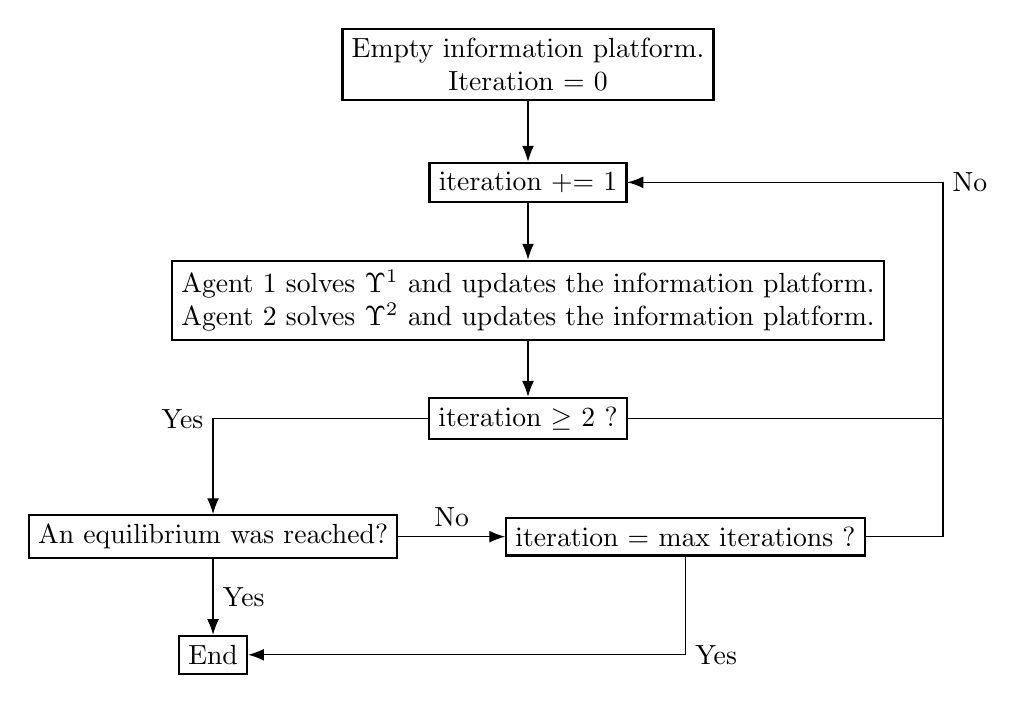
\begin{tikzpicture}
\begin{scope}[every node/.style={rectangle,draw,thick}]
	\node[align = center] (init) at (0,0)  {Empty information platform.\\
	Iteration = 0};
	\node (iteration) at (0,-1.5){iteration += 1};
	\node[align =left] (main) at (0,-3) {Agent 1 solves $\Upsilon^1$  and updates the information platform.\\
	Agent 2 solves $\Upsilon^2$  and updates the information platform.};
	\node (itquestion) at (0,-4.5) {iteration $\geq$ 2 ?};

	\node (equiquestion) at (-4,-6) {An equilibrium was reached?};

	\node (maxit) at (2,-6) {iteration = max iterations ?};

	\node (End) at (-4,-7.5) {End};
\end{scope}

\begin{scope}
	\draw[-{Latex[length=2mm]}] (init) edge (iteration);
	\draw[-{Latex[length=2mm]}] (iteration) edge (main);
	\draw[-{Latex[length=2mm]}] (main) edge (itquestion);
	\draw[-{Latex[length=2mm]}] (itquestion.east)  -- ++(4cm,0) |- node[right] {No}
	 (iteration.east);
	\draw[-{Latex[length=2mm]}] (itquestion.west) -| node[left] {Yes} (equiquestion);
	\draw[-{Latex[length=2mm]}] (equiquestion)  edge node[above] {No} (maxit);
	\draw[-{Latex[length=2mm]}] (equiquestion) edge node[right] {Yes} (End);
	\draw[-{Latex[length=2mm]}] (maxit.south) |- node[right] {Yes} (End);
	\draw[-] (maxit.east)  -- ++(0.98cm,0) |- (iteration.east);




\end{scope}

\end{tikzpicture}
\end{figure}

\section{Results} \label{seq:results}

\subsection{Comparision 3 centralized mechanisms}

\subsection{Comparision centralized mechanisms and iterative one, all for 2 agents}

Here

\begin{table}[ht!]
\caption{Analysis of the impact of the order of the agents in the iterative mechanism \label{tb:iter_order_comparition}}
\begin{tabular}{lrrrrrr}
\toprule
{} &  Order1\_payoff &  Order2\_payoff &      Dif\% &  Order1\_it &  Order2\_it &  Dif\_it \\
\midrule
2\_low\_0  &           25.0 &           25.0 &  0.00 &        4.0 &        3.0 &     1.0 \\
2\_low\_1  &           21.0 &           21.0 &  0.00 &        3.0 &        3.0 &     0.0 \\
2\_low\_2  &           17.0 &           17.0 &  0.00 &        3.0 &        3.0 &     0.0 \\
2\_low\_3  &           15.0 &           15.0 &  0.00 &        4.0 &        4.0 &     0.0 \\
2\_low\_4  &           27.0 &           26.0 &  3.70 &        3.0 &        3.0 &     0.0 \\
2\_high\_0 &           73.0 &           72.0 &  1.37 &        3.0 &        3.0 &     0.0 \\
2\_high\_1 &           70.0 &           69.0 &  1.49 &        3.0 &        3.0 &     0.0 \\
2\_high\_2 &           65.0 &           63.0 &  3.08 &        3.0 &        3.0 &     0.0 \\
2\_high\_3 &           68.0 &           67.0 &  1.47 &        4.0 &        4.0 &     0.0 \\
2\_high\_4 &           74.0 &           73.0 &  1.35 &        3.0 &        3.0 &     0.0 \\
\bottomrule
\end{tabular}
\end{table}

Here
\section{Discussion} \label{seq:discussion}

\section{Conclusion} \label{seq:conclusion}


\bibliography{bibliography}

\appendix
\section{ILP's}
\label{seq:appendixilp}

\subsection{ILP to be solved by the central planner in the centralized full cooperation scenario.}

    \begin{align}
        &  \Gamma_F: \max  & \hspace{22pt} \sum_{(o,t,i)\in \Theta} \sum_{e \in \delta^-(t)\cap E}  f_e^{(o,t,i)} \cdot d_{(o,t,i)} \cdot r_{(o,t,i)} - \sum_{e\in E} u_{e}\cdot c_{e} \hspace{40pt} && 
    \end{align}
    \begin{align}
        & \text{subject to:}       && \nonumber \\
        & \sum_{e \in \delta^-(z)\cap E} f_e^{(o,t,i)} -\sum_{e \in \delta^+(z)\cap E} f_{e}^{(o,t,i)} = 0,\quad && \forall\ z\in V\setminus\{o,t\},\ \forall\ (o,t,i)\in\Theta, \\
& \sum_{e \in \delta^+(o)\cap E} f_e^{(o,t,i)} \leq 1, && \forall\ (o,t,i)\in \Theta, \\
 & \sum_{e \in \delta^+(t)\cap E} f_e^{(o,t,i)} = 0,  && \forall\ (o,t,i)\in \Theta,  \\
& \sum_{(o,t,i) \in \Theta} f_e^{(o,t,i)}\cdot d_{(o,t,i)}  \leq u_e\cdot q_e, && \forall\ e \in E,   \\
 & \sum_{\substack{(v,w,k) \in E\colon \\ v,w \in S}} f_{(v,w,k)}^{(o,t,i)} \leq |S| -1, && \forall\ S \subset V,\ \forall\ (o,t,i) \in \Theta,\\
&\sum_{e \in \delta^-(t)\cap E}  f_e^{(o,t,i)}  \cdot d_{(o,t,i)} \cdot r_{(o,t,i)} - && \nonumber\\
& -\sum_{\substack{e \in E^j\colon \\ j\not = i}} f_e^{(o,t,i)} \cdot d_{(o,t,i)} \cdot \frac{c_e}{q_e}\geq 0, && \forall\ (o,t,i) \in \Theta, \\
& \varphi_i(\Gamma_F) \geq P_i^*,  && \forall\ i\in N, \\
& f_e^{(o,t,i)} \in \{0,1\},  && \forall\ e \in E,\ \forall\ (o,t,i) \in \Theta,  \\
&  u_e  \in \{0,1\},  && \forall\ e \in E.
    \end{align}

\subsection{ILP to be solved by the central planner in the centralized residual cooperation scenario.}

  \begin{align}
        &  \Gamma_R: \max  & \sum_{(o,t,i) \in \Theta_R} \sum_{e \in \delta^-(t)\cap E_R}  f_e^{(o,t,i)} \cdot d_{(o,t,i)} \cdot r_{(o,t,i)} &&   
    \end{align}
    \begin{align}
        & \text{subject to:}       && \nonumber\\
        & \sum_{e \in \delta^-(z)\cap E_R} f_e^{(o,t,i)}-\sum_{e \in \delta^+(z)\cap E_R} f_{e}^{(o,t,i)}  = 0,           \quad && \forall\ z\in V\setminus\{o,t\},\ \forall\ (o,t,i)\in\Theta_R, \\[1em]
& \sum_{e \in \delta^+(o)\cap E_R} f_e^{(o,t,i)}\leq 1, && \forall\ (o,t,i)\in \Theta_R,  \\
& \sum_{e \in \delta^+(t)\cap E_R} f_e^{(o,t,i)}  = 0, && \forall\ (o,t,i)\in \Theta_R,  \\
 & \sum_{(o,t,i) \in \Theta_R} f_e^{(o,t,i)}\cdot d_{(o,t,i)} \leq q_e^R   &&\forall\ e \in E_R,   \\
& \sum_{\substack{(v,w,k)\in E_R\colon\\v\in S,w \in S }} f_{(v,w,k)}^{(o,t,i)} \leq |S| -1,  && \forall\ S \subset V, \ \forall\ (o,t,i) \in \Theta_R, \\
& \sum_{e \in \delta^-(t)\cap E_R}  f_e^{(o,t,i)}  \cdot d_{(o,t,i)} \cdot r_{(o,t,i)} - && \nonumber\\
& -\sum_{\substack{e \in E_R^j\colon \\ j\not = i}} f_e^{(o,t,i)} \cdot d_{(o,t,i)} \cdot \frac{c_e}{q_e}\geq 0, && \forall\ (o,t,i) \in \Theta_R, \\
& f_e^{(o,t,i)} \in \{0,1\},    && \forall\ e \in E_R, \forall\ (o,t,i) \in \Theta_R.
    \end{align}

\end{document}